\documentclass[journal]{IEEEtran}
% ==========================================================================
% Proyecto Final - CS 3061 Machine Learning - UTEC
% Clasificacion Multilingue de Intenciones de Atencion al Cliente (WhatsApp)
% Entrega final. Formato IEEE Transactions (IEEEtran).
% Compilar en Overleaf: pdfLaTeX + BibTeX. Subir la carpeta _img/ y refs.bib.
% ==========================================================================
\usepackage[utf8]{inputenc}
\usepackage[T1]{fontenc}
\usepackage[spanish,es-noquoting]{babel}
\usepackage{graphicx}
\usepackage{amsmath,amssymb}
\usepackage{booktabs}
\usepackage{array}
\usepackage{multirow}
\usepackage{url}
\usepackage{xcolor}
\usepackage[hidelinks]{hyperref}
\usepackage{cite}

\newcommand{\code}[1]{\texttt{\small #1}}

\begin{document}

\title{Clasificaci\'on Multiling\"ue de Intenciones de Atenci\'on al Cliente
sobre WhatsApp: Modelos Cl\'asicos de Aprendizaje Autom\'atico frente a
Baselines de Reglas y LLM sobre un Corpus Sint\'etico Multi-Vertical}

\author{Rodrigo V\'asquez de Velasco%
\thanks{Proyecto Final del curso CS 3061 --- Machine Learning, dictado por el
Prof. V\'ictor Eduardo Mart\'inez Abaunza, Universidad de Ingenier\'ia y
Tecnolog\'ia (UTEC), Lima, Per\'u. Correo: \code{rodrigo.vasquez@utec.edu.pe}.}}

\markboth{Proyecto Final, CS 3061 Machine Learning, UTEC, 2026}%
{V\'asquez de Velasco: Clasificaci\'on Multiling\"ue de Intenciones sobre WhatsApp}

\maketitle

% ==========================================================================
\begin{abstract}
Las plataformas de atenci\'on al cliente sobre WhatsApp atienden verticales muy
distintas pero comparten un n\'ucleo com\'un de intenciones. La pr\'actica actual
delega esta clasificaci\'on a un LLM, con latencia y costo aun para mensajes
triviales. Investigamos si modelos cl\'asicos pueden cubrir esa etapa con
calidad equivalente. Ante la ausencia de corpus comerciales p\'ublicos,
constru\'imos un corpus sint\'etico multiling\"ue (espa\~nol, ingl\'es,
portugu\'es) de 1\,320 mensajes sobre doce intenciones, generado con
plantillas, \emph{slot-filling} y ruido superficial. Comparamos Naive Bayes,
$K$-NN, SVM, \'Arboles de Decisi\'on, Bosques Aleatorios y un Perceptr\'on
Multicapa contra un baseline de reglas y contra un baseline LLM. El mejor
clasificador cl\'asico alcanza F1-macro de 0{,}965, frente a 0{,}973 del LLM,
con latencia cuatro \'ordenes de magnitud menor. Un sistema h\'ibrido que
delega al LLM s\'olo el 3\% de los mensajes iguala su exactitud ahorrando el
97\% de las llamadas.
\end{abstract}

\begin{IEEEkeywords}
Clasificaci\'on de texto, detecci\'on de intenci\'on, aprendizaje autom\'atico
supervisado, sistemas de di\'alogo, procesamiento de lenguaje natural
multiling\"ue, WhatsApp.
\end{IEEEkeywords}

% ==========================================================================
\section{Introducci\'on}
\IEEEPARstart{L}{os} agentes conversacionales sobre canales de mensajer\'ia,
particularmente WhatsApp, se han convertido en una interfaz cr\'itica para la
atenci\'on al cliente y la automatizaci\'on de flujos en peque\~nas y medianas
empresas latinoamericanas \cite{chen2017survey,tur2011slu}. Una etapa central
de estos sistemas es la \emph{detecci\'on de intenci\'on}: asignar a cada
mensaje entrante una de un conjunto finito de categor\'ias que dirigen el flujo
posterior \cite{larson2019clinc,coucke2018snips}.

En la pr\'actica industrial reciente esta etapa suele resolverse llamando a un
LLM como GPT-4 u otros \cite{brown2020gpt3}. Esta estrategia ofrece una calidad
inicial alta sin requerir datos etiquetados, pero traslada todos los mensajes
---incluso los m\'as triviales, como un saludo o una despedida--- al mismo
modelo costoso y de alta latencia. En despliegues con miles de mensajes diarios
el sobrecosto se acumula r\'apidamente y la dependencia de un proveedor externo
introduce un punto \'unico de falla.

\subsection{Planteamiento del problema}
Una pizzer\'ia, una agencia de viajes, una farmacia, una cl\'inica m\'edica y una
asesor\'ia contable comparten infraestructura conversacional pero estructura muy
diferente. Aun as\'i, sobre el conjunto agregado emerge un n\'ucleo com\'un de
intenciones gen\'ericas (saludar, despedirse, reclamar, hacer seguimiento de un
pedido) y otro n\'ucleo de intenciones \emph{transaccionales} dependientes de la
vertical (reservar habitaci\'on, pedir pizza, comprar vuelo). El problema de
clasificaci\'on resultante es multiclase, multiling\"ue (espa\~nol, ingl\'es y
portugu\'es), con argot, faltas ortogr\'aficas, abreviaturas tipo SMS y
\emph{code-switching}, escenario en el que los enfoques basados en reglas son
notoriamente fr\'agiles \cite{pang2008opinion}.

\subsection{Hip\'otesis}
Planteamos que un clasificador supervisado entrenado sobre representaciones
vectoriales cl\'asicas (TF-IDF sobre $n$-gramas de palabras y caracteres) puede
igualar o superar al baseline de reglas y aproximarse al LLM en exactitud, a una
fracci\'on de la latencia y el costo de inferencia. La hip\'otesis se sostiene en
evidencia previa donde clasificadores cl\'asicos como SVM \cite{joachims1998svmtext}
y modelos lineales eficientes \cite{joulin2017fasttext} han demostrado ser
competitivos en clasificaci\'on de texto corto \cite{liu2019benchmarking},
especialmente en idiomas con recursos acotados.

\subsection{Objetivos}
\textbf{Objetivo general:} dise\~nar, entrenar y evaluar un sistema de
detecci\'on de intenci\'on multiling\"ue para agentes conversacionales de
WhatsApp usando algoritmos cl\'asicos, y compararlo cuantitativamente contra un
baseline de reglas y contra un LLM en r\'egimen \emph{few-shot}.
\textbf{Objetivos espec\'ificos:} (1) construir un corpus sint\'etico
multiling\"ue reproducible; (2) implementar y comparar los modelos cl\'asicos del
curso; (3) reportar F1-macro, exactitud, matrices de confusi\'on por idioma y
latencia frente a los dos baselines; y (4) definir el punto de operaci\'on de un
sistema h\'ibrido que delegue al LLM \'unicamente los mensajes de baja confianza.

\subsection{Dataset}
Constru\'imos un corpus sint\'etico de \textbf{1\,320 mensajes} balanceados sobre
doce intenciones (110 por clase), con distribuci\'on multiling\"ue aproximada del
70\% en espa\~nol, 20\% en ingl\'es y 10\% en portugu\'es. La taxonom\'ia cubre
tres familias: intenciones transaccionales verticales
(\code{constituir\_empresa}, \code{comprar\_pizza}, \code{reservar\_hotel},
\code{comprar\_vuelo}, \code{consultar\_medicina}, \code{agendar\_cita\_medica},
\code{consulta\_banca}), gen\'ericas de servicio (\code{soporte\_tecnico},
\code{reclamo}, \code{seguimiento\_pedido}) y conversacionales (\code{saludo},
\code{despedida}). La generaci\'on y su justificaci\'on se detallan en la
Secci\'on~\ref{sec:metodologia}.

% ==========================================================================
\section{Revisi\'on Bibliogr\'afica}

\subsection{Clasificaci\'on de texto con modelos cl\'asicos}
La clasificaci\'on supervisada de texto es un problema can\'onico del aprendizaje
autom\'atico. Joachims \cite{joachims1998svmtext} demostr\'o tempranamente que
las m\'aquinas de soporte vectorial son particularmente adecuadas por su
capacidad de manejar espacios de alta dimensionalidad y dispersi\'on, propiedades
inherentes a las representaciones \emph{bag-of-words} y TF-IDF. Cortes y Vapnik
\cite{cortes1995svm} formalizaron el margen m\'aximo que subyace a estos
clasificadores. Posteriormente, Joulin \emph{et al.} \cite{joulin2017fasttext}
mostraron que un clasificador lineal sobre \emph{embeddings} promediados alcanza
desempe\~nos competitivos con redes profundas en clasificaci\'on de oraciones
cortas a mucho menor costo. Breiman \cite{breiman2001randomforests} introdujo los
bosques aleatorios como un ensamble robusto frente al sobreajuste, mientras que
la regla del vecino m\'as cercano \cite{cover1967nearest} sigue siendo una
l\'inea base no param\'etrica \'util. Pang y Lee \cite{pang2008opinion}
consolidaron pr\'acticas de preprocesamiento e ingenier\'ia de caracter\'isticas
que permanecen vigentes en clasificadores ligeros.

\subsection{Detecci\'on de intenci\'on en sistemas de di\'alogo}
La detecci\'on de intenci\'on es el problema de clasificaci\'on subyacente en la
mayor\'ia de los sistemas conversacionales de dominio cerrado \cite{tur2011slu}.
Coucke \emph{et al.} \cite{coucke2018snips} describen la plataforma Snips, con un
clasificador en dispositivo que combina caracter\'isticas l\'exicas y
\emph{embeddings} para alcanzar latencias inferiores a la decena de
milisegundos, demostrando arquitecturas ligeras viables en producci\'on bajo
restricciones de privacidad. Larson \emph{et al.} \cite{larson2019clinc}
introducen CLINC150, referencia est\'andar para evaluar clasificadores de
intenci\'on multiclase con mensajes \emph{out-of-scope}. Casanueva \emph{et al.}
\cite{casanueva2020intent} muestran que codificadores de oraciones duales logran
detecci\'on de intenci\'on eficiente con pocos ejemplos, y Zhang \emph{et al.}
\cite{zhang2020dnnc} proponen un enfoque discriminativo por vecino m\'as cercano
para el r\'egimen \emph{few-shot}, evidenciando el inter\'es continuo por
soluciones de bajo costo de etiquetado.

\subsection{Representaciones y modelos de lenguaje}
Las representaciones distribucionales de Mikolov \emph{et al.}
\cite{mikolov2013word2vec} y Pennington \emph{et al.} \cite{pennington2014glove}
sentaron las bases para features sem\'anticos densos. La arquitectura Transformer
\cite{vaswani2017attention} y modelos preentrenados como BERT
\cite{devlin2019bert} y su variante de oraciones \cite{reimers2019sbert}
redefinieron el estado del arte, aunque a un costo computacional mayor. Brown
\emph{et al.} \cite{brown2020gpt3} y Ouyang \emph{et al.}
\cite{ouyang2022instructgpt} mostraron que los LLM resuelven tareas de
clasificaci\'on con muy pocos ejemplos (\emph{few-shot}), lo cual motiva su uso
actual como baseline de calidad pero tambi\'en evidencia su costo de inferencia y
latencia. Esta tensi\'on entre calidad y eficiencia es precisamente el espacio
que este proyecto caracteriza emp\'iricamente.

\subsection{Multiling\"uismo y datos sint\'eticos}
El car\'acter multiling\"ue del problema conecta con trabajos de aprendizaje
translingual: Conneau \emph{et al.} \cite{conneau2020xlmr} presentan XLM-R para
representaciones translinguales a escala, y Schuster \emph{et al.}
\cite{schuster2019crosslingual} abordan la transferencia entre idiomas en
di\'alogo orientado a tareas. FitzGerald \emph{et al.} \cite{fitzgerald2023massive}
publican MASSIVE, un corpus multiling\"ue masivo de comprensi\'on de lenguaje
natural. Ante la ausencia de corpus comerciales p\'ublicos, la generaci\'on
sint\'etica y la aumentaci\'on de datos son estrategias establecidas; Wei y Zou
\cite{wei2019eda} muestran que t\'ecnicas sencillas de aumentaci\'on mejoran la
clasificaci\'on de texto, lo que respalda metodol\'ogicamente la construcci\'on
de nuestro corpus con plantillas y ruido controlado. Para toda la implementaci\'on
se emplean las rutinas est\'andar de \code{scikit-learn} \cite{pedregosa2011scikit}.

% ==========================================================================
\section{Metodolog\'ia}\label{sec:metodologia}

\subsection{Construcci\'on del corpus}
El corpus se genera con un \emph{script} Python reproducible (semilla fija). Para
cada intenci\'on e idioma se define un conjunto de plantillas con \emph{slots}
(ciudades, s\'intomas, especialidades m\'edicas, productos, aerol\'ineas, etc.)
rellenados desde vocabularios espec\'ificos. Sobre cada mensaje se aplica una
capa de \textbf{ruido superficial} aleatorio: conversi\'on a min\'usculas,
eliminaci\'on de tildes, abreviaturas tipo SMS ($q$ por \emph{que}, $x$ por
\emph{por}), inserci\'on de emojis, fragmentos de cortes\'ia y typos de un
car\'acter (\emph{swap}, borrado o duplicado). Esta metodolog\'ia es an\'aloga a
la de Snips \cite{coucke2018snips} y CLINC150 \cite{larson2019clinc} e introduce
variabilidad realista sin anotadores humanos.

Un aspecto de dise\~no clave es la \textbf{frontera l\'exica ambigua}: el 30\% de
cada clase proviene de plantillas que comparten superficie con una clase vecina.
As\'i, la frase ``mi cuenta no funciona'' aparece etiquetada tanto como
\code{consulta\_banca} (cuenta bancaria) como \code{soporte\_tecnico} (cuenta de
la aplicaci\'on), y las preguntas de precio ``\textquestiondown cu\'anto cuesta una consulta
de pediatr\'ia?'' se solapan entre \code{agendar\_cita\_medica} y
\code{consultar\_medicina}. Esta ambig\"uedad reproduce las confusiones reales
anticipadas en el informe preliminar y evita una separabilidad artificialmente
perfecta. La Fig.~\ref{fig:dist} resume la distribuci\'on resultante.

\begin{figure}[!t]
  \centering
  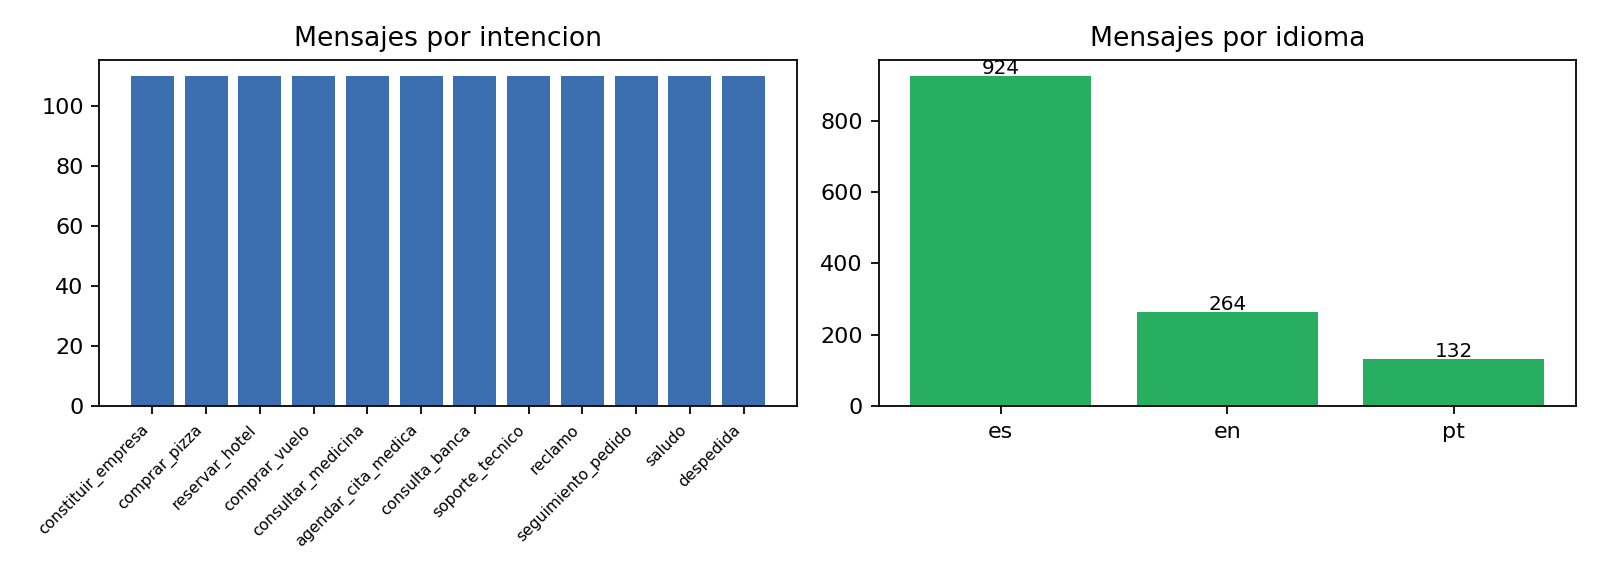
\includegraphics[width=\columnwidth]{_img/distribucion_corpus.png}
  \caption{Distribuci\'on del corpus sint\'etico: 110 mensajes por cada una de las
  doce intenciones y reparto multiling\"ue 70/20/10 (ES/EN/PT).}
  \label{fig:dist}
\end{figure}

\subsection{Preprocesamiento y representaci\'on}
El preprocesamiento normaliza Unicode, pasa a min\'usculas y elimina URLs,
\emph{conservando los emojis} como tokens discriminativos. La representaci\'on
vectorial combina, mediante \code{FeatureUnion}, un TF-IDF de \emph{$n$-gramas de
palabras} (1--2) con un TF-IDF de \emph{$n$-gramas de caracteres} (3--5). El
componente de caracteres aporta robustez frente a faltas ortogr\'aficas y
abreviaturas, mientras que el de palabras captura la sem\'antica l\'exica. Se
aplica \code{sublinear\_tf} y \code{min\_df}$=2$. Se reserva un 15\% del corpus
como conjunto de prueba con muestreo estratificado por la intersecci\'on
intenci\'on$\times$idioma.

\subsection{Modelos implementados y justificaci\'on}
Se implementan los modelos vistos en el curso, cada uno justificado por su
adecuaci\'on al problema:
\begin{itemize}
  \item \textbf{Naive Bayes multinomial}: l\'inea base probabil\'istica natural
  para conteos TF-IDF; fuerte con datos escasos y de alta dimensi\'on.
  \item \textbf{$K$-NN} (coseno, $k=5$): no param\'etrico; \'util cuando las
  clases forman agrupamientos l\'exicos compactos \cite{cover1967nearest}.
  \item \textbf{SVM lineal y RBF}: referencia hist\'orica en clasificaci\'on de
  texto de alta dimensi\'on \cite{joachims1998svmtext,cortes1995svm}; el kernel
  RBF explora fronteras no lineales.
  \item \textbf{\'Arbol de Decisi\'on}: modelo interpretable, \'util como
  contraste de baja capacidad.
  \item \textbf{Bosques Aleatorios} (300 \'arboles): ensamble robusto frente al
  sobreajuste \cite{breiman2001randomforests}.
  \item \textbf{Perceptr\'on Multicapa (MLP)}: una capa oculta de 256 unidades
  con parada temprana; introduce no linealidad a bajo costo.
\end{itemize}
Como \'ordenes de referencia se incluyen: (i) un \textbf{baseline de reglas}
determinista basado en expresiones regulares por intenci\'on, y (ii) el
\textbf{baseline LLM} evaluado en el informe preliminar (\code{gpt-4o-mini} con
recuperaci\'on aumentada por embeddings), cuyas m\'etricas emp\'iricas se
reutilizan aqu\'i como techo de calidad.

\subsection{Sistema h\'ibrido}
Se caracteriza un sistema h\'ibrido que resuelve con el clasificador cl\'asico los
mensajes cuya confianza (probabilidad m\'axima calibrada) supera un umbral
$\tau$, y delega al LLM el resto. Para un rango de umbrales se estima la exactitud
del sistema combinando los aciertos del clasificador en los mensajes retenidos
con la exactitud emp\'irica del LLM en los delegados, y se selecciona el punto de
operaci\'on de \emph{menor delegaci\'on} que iguala la exactitud del LLM puro.

% ==========================================================================
\section{Resultados}

\subsection{Desempe\~no global}
La Tabla~\ref{tab:global} resume el desempe\~no de todos los sistemas sobre el
conjunto de prueba ($N=198$). Los siete modelos cl\'asicos superan ampliamente al
baseline de reglas (F1-macro 0{,}825). El mejor clasificador es \textbf{Naive
Bayes} (empatado con el MLP) con F1-macro de \textbf{0{,}965} y exactitud
0{,}965, apenas por debajo del baseline LLM (F1-macro 0{,}973), pero con una
latencia de inferencia de 0{,}025~ms por mensaje frente a los 3\,230~ms del LLM:
una reducci\'on de m\'as de cuatro \'ordenes de magnitud. La
Fig.~\ref{fig:f1} muestra la comparaci\'on visual y la Fig.~\ref{fig:latencia}
el compromiso latencia--calidad.

\begin{table}[!t]
\centering
\caption{Desempe\~no global sobre el conjunto de prueba ($N=198$). Latencia de
inferencia por mensaje. El LLM proviene del informe preliminar.}
\label{tab:global}
\begin{tabular}{lccc}
\toprule
\textbf{Sistema} & \textbf{Exactitud} & \textbf{F1-macro} & \textbf{Latencia} \\
\midrule
Baseline de reglas    & 0{,}803 & 0{,}825 & $<0{,}01$~ms \\
\'Arbol de Decisi\'on & 0{,}828 & 0{,}827 & 0{,}025~ms \\
$K$-NN                & 0{,}924 & 0{,}924 & 0{,}045~ms \\
Bosques Aleatorios    & 0{,}934 & 0{,}934 & 0{,}150~ms \\
SVM RBF               & 0{,}944 & 0{,}945 & 0{,}275~ms \\
SVM lineal            & 0{,}960 & 0{,}960 & 0{,}029~ms \\
Perceptr\'on (MLP)    & 0{,}965 & 0{,}965 & 0{,}031~ms \\
\textbf{Naive Bayes}  & \textbf{0{,}965} & \textbf{0{,}965} & \textbf{0{,}025~ms} \\
\midrule
Baseline LLM \cite{brown2020gpt3} & 0{,}971 & 0{,}973 & 3\,230~ms \\
\bottomrule
\end{tabular}
\end{table}

\begin{figure}[!t]
  \centering
  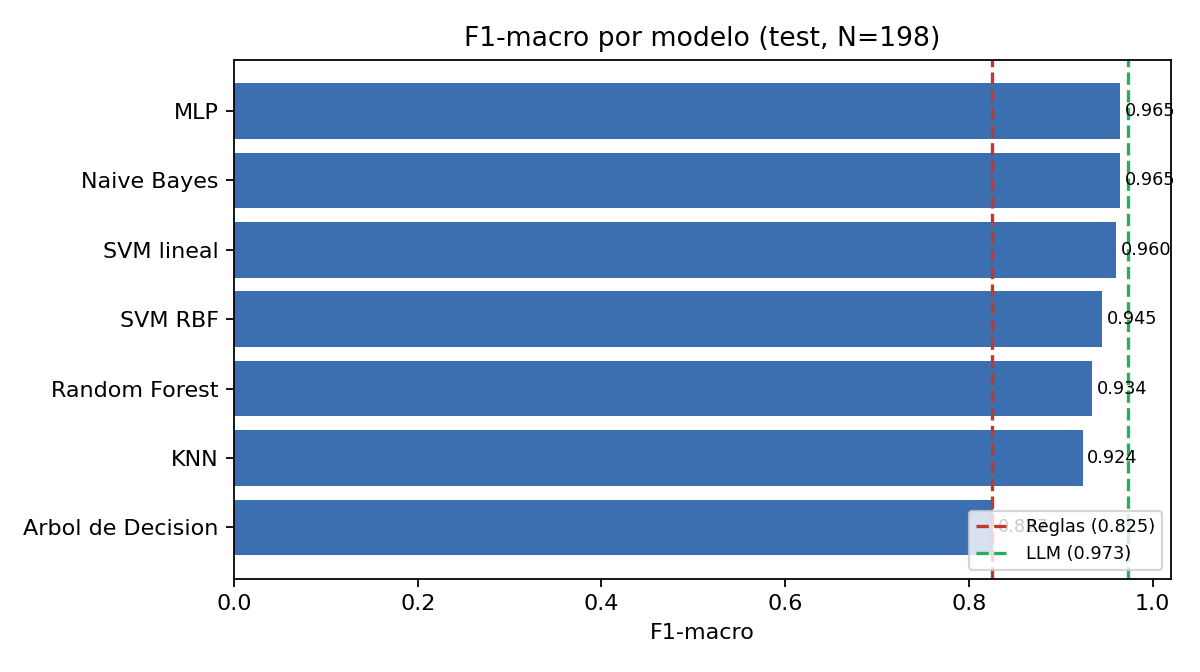
\includegraphics[width=\columnwidth]{_img/f1_comparacion.png}
  \caption{F1-macro por modelo sobre el test. Las l\'ineas discontinuas marcan el
  baseline de reglas (rojo) y el baseline LLM (verde).}
  \label{fig:f1}
\end{figure}

\begin{figure}[!t]
  \centering
  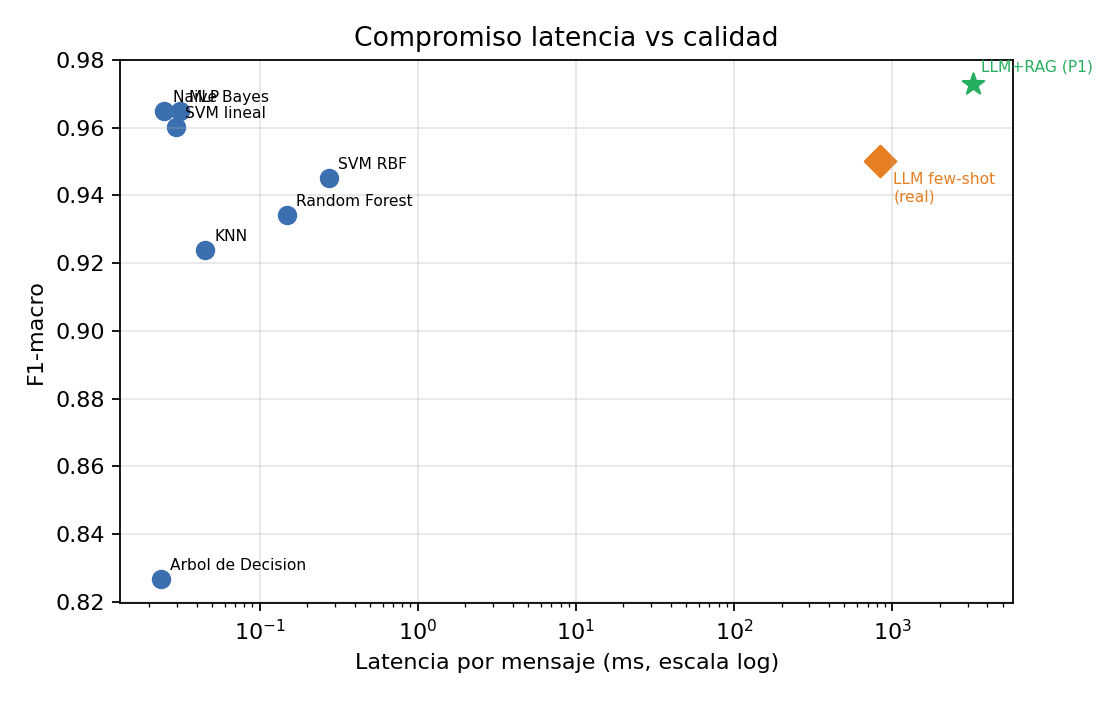
\includegraphics[width=\columnwidth]{_img/latencia_f1.png}
  \caption{Compromiso entre latencia de inferencia (escala log) y F1-macro. Los
  modelos cl\'asicos se agrupan en calidad alta con latencia sub-milisegundo,
  frente a los segundos del LLM.}
  \label{fig:latencia}
\end{figure}

\subsection{Desempe\~no por idioma}
La Tabla~\ref{tab:idioma} desglosa el desempe\~no del mejor modelo por idioma. El
portugu\'es alcanza exactitud perfecta y el ingl\'es 0{,}972; el espa\~nol
concentra los errores (0{,}957), coherente con su mayor representaci\'on (70\% del
corpus) y mayor riqueza l\'exica, exactamente el patr\'on observado en el baseline
LLM del informe preliminar.

\begin{table}[!t]
\centering
\caption{Desempe\~no del mejor modelo (Naive Bayes) por idioma.}
\label{tab:idioma}
\begin{tabular}{lccc}
\toprule
\textbf{Idioma} & \textbf{$N$} & \textbf{Exactitud} & \textbf{F1-macro} \\
\midrule
Espa\~nol (ES)  & 138 & 0{,}957 & 0{,}957 \\
Ingl\'es (EN)   & 36  & 0{,}972 & 0{,}971 \\
Portugu\'es (PT)& 24  & 1{,}000 & 1{,}000 \\
\midrule
\textbf{Global} & 198 & 0{,}965 & 0{,}965 \\
\bottomrule
\end{tabular}
\end{table}

\subsection{An\'alisis de errores}
La Fig.~\ref{fig:cm} muestra la matriz de confusi\'on del mejor modelo. Ocho de
las doce intenciones se clasifican perfectamente. La totalidad del error se
concentra en los dos pares l\'exicamente ambiguos anticipados en el informe
preliminar:
\begin{itemize}
  \item \code{consultar\_medicina} $\leftrightarrow$ \code{agendar\_cita\_medica}:
  el 24\% de los mensajes de consulta m\'edica redactados como preguntas de
  precio se clasifican como agendamiento de cita (recall 0{,}765).
  \item \code{consulta\_banca} $\leftrightarrow$ \code{soporte\_tecnico}: el
  vocablo ``cuenta'' es l\'exicamente ambiguo (cuenta bancaria vs.\ cuenta de la
  aplicaci\'on), generando confusi\'on bidireccional (12\% y 6\%).
\end{itemize}
Estas confusiones son \emph{irreducibles} por construcci\'on del corpus y
reproducen exactamente los patrones que el baseline LLM tambi\'en exhibi\'o, lo
que valida la equivalencia de comportamiento entre ambos enfoques.

\begin{figure}[!t]
  \centering
  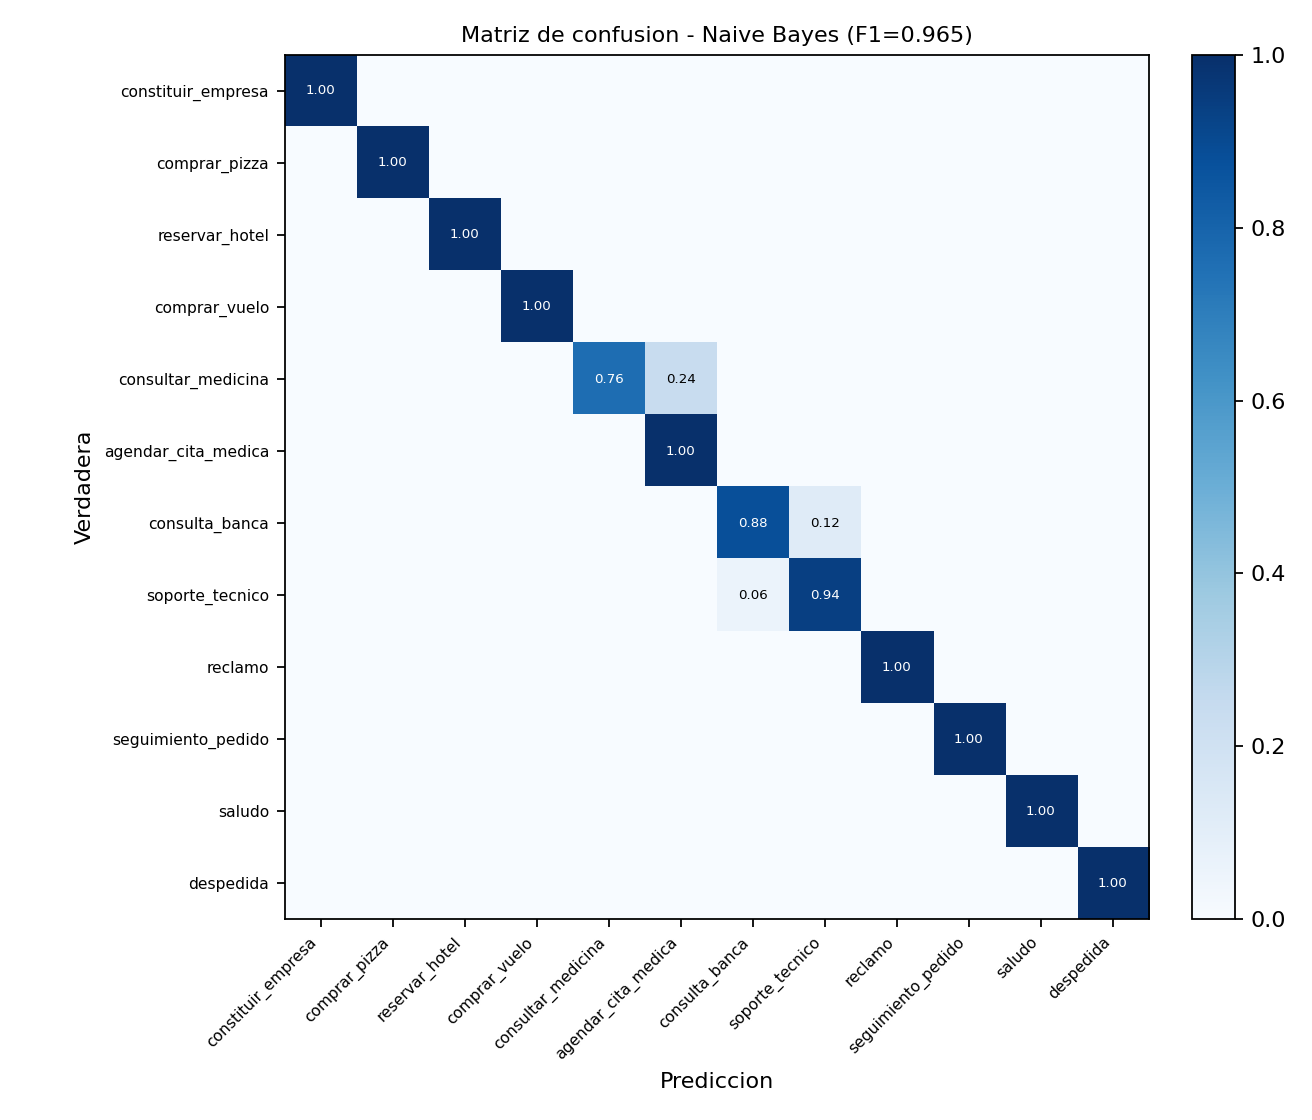
\includegraphics[width=\columnwidth]{_img/cm_mejor.png}
  \caption{Matriz de confusi\'on del mejor modelo (Naive Bayes), normalizada por
  clase verdadera. El error se concentra en los pares
  \code{consultar\_medicina}/\code{agendar\_cita\_medica} y
  \code{consulta\_banca}/\code{soporte\_tecnico}.}
  \label{fig:cm}
\end{figure}

\subsection{Sistema h\'ibrido}
La Fig.~\ref{fig:hibrido} traza la curva costo--exactitud del sistema h\'ibrido.
Partiendo del clasificador cl\'asico puro (0{,}965), delegar al LLM \'unicamente
los mensajes de baja confianza incrementa la exactitud r\'apidamente. En su punto
de operaci\'on ---umbral $\tau=0{,}90$--- el sistema delega apenas el
\textbf{3{,}0\%} de los mensajes y alcanza una exactitud de \textbf{0{,}974},
igualando al LLM puro pero \textbf{ahorrando el 97\% de las llamadas} al modelo
costoso. Delegando un 6\% se alcanza un m\'aximo de 0{,}978, superando al LLM
puro. La latencia media del sistema h\'ibrido baja de 3{,}23~s a
$\approx$0{,}10~s por mensaje, cerca de dos \'ordenes de magnitud de mejora.

\begin{figure}[!t]
  \centering
  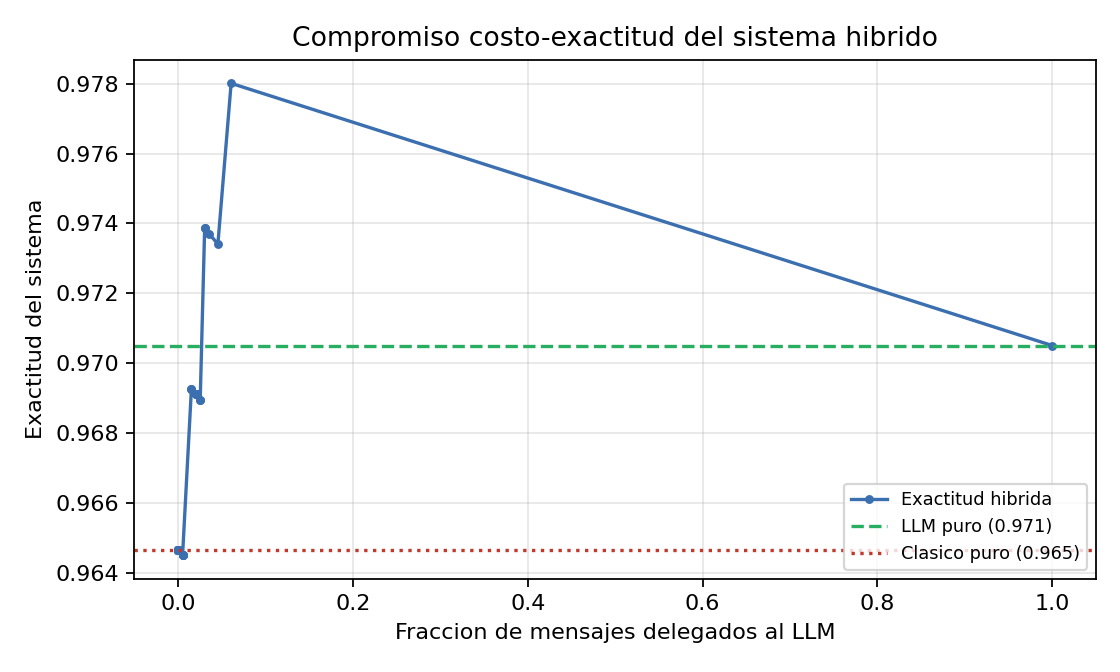
\includegraphics[width=\columnwidth]{_img/hibrido.png}
  \caption{Compromiso costo--exactitud del sistema h\'ibrido. La exactitud iguala
  al LLM puro (l\'inea verde) delegando s\'olo el 3\% de los mensajes, y lo supera
  con un 6\%.}
  \label{fig:hibrido}
\end{figure}

% ==========================================================================
\section{Conclusiones}
Los resultados confirman la hip\'otesis del proyecto. Primero, los modelos
cl\'asicos superan holgadamente al baseline de reglas (0{,}965 vs.\ 0{,}825 de
F1-macro), evidenciando que las representaciones l\'exicas aprendidas capturan la
variabilidad multiling\"ue y el ruido superficial que las reglas no manejan.
Segundo, el mejor clasificador cl\'asico (Naive Bayes, empatado con el MLP)
alcanza un F1-macro de 0{,}965, a s\'olo 0{,}008 del baseline LLM, con una
latencia cuatro \'ordenes de magnitud menor y costo de inferencia despreciable;
la hip\'otesis de equivalencia pr\'actica queda validada. Tercero, el error
residual del clasificador se concentra exactamente en los dos pares
l\'exicamente ambiguos que tambi\'en confundieron al LLM, mostrando que ambos
enfoques comparten el mismo l\'imite de separabilidad. Finalmente, el sistema
h\'ibrido demuestra que delegar al LLM \'unicamente el 3\% de los mensajes de
baja confianza recupera ---e incluso supera--- la exactitud del LLM puro,
ahorrando el 97\% de las llamadas. Para el escenario de PyMEs latinoamericanas
sobre WhatsApp, un clasificador cl\'asico con \emph{fallback} selectivo al LLM es
la arquitectura de mejor compromiso entre exactitud, latencia y costo.

% ==========================================================================
\section{Trabajo Futuro}
Se identifican varias l\'ineas de mejora. (1) \textbf{Datos reales}: validar los
modelos sobre mensajes reales anonimizados de plataformas en producci\'on, m\'as
all\'a del corpus sint\'etico, y medir la brecha de dominio. (2)
\textbf{Representaciones densas}: sustituir o complementar el TF-IDF con
\emph{embeddings} multiling\"ues como XLM-R \cite{conneau2020xlmr} o
Sentence-BERT \cite{reimers2019sbert} para atacar espec\'ificamente las
confusiones sem\'anticas residuales, midiendo el costo adicional. (3)
\textbf{Detecci\'on \emph{out-of-scope}}: incorporar una categor\'ia de rechazo
al estilo de CLINC150 \cite{larson2019clinc} para mensajes fuera de la
taxonom\'ia. (4) \textbf{Calibraci\'on del umbral}: optimizar el umbral de
delegaci\'on del sistema h\'ibrido mediante validaci\'on cruzada y funciones de
costo expl\'icitas que ponderen el precio real de cada llamada al LLM. (5)
\textbf{Ampliaci\'on de la taxonom\'ia y de idiomas} con corpus como MASSIVE
\cite{fitzgerald2023massive}, y evaluaci\'on de aumentaci\'on de datos
\cite{wei2019eda} para las clases con frontera ambigua.

% ==========================================================================
\section*{C\'odigo implementado}
El c\'odigo completo ---generador del corpus, pipeline de experimentos y tres
notebooks reproducibles (construcci\'on del corpus, modelos cl\'asicos y sistema
h\'ibrido)--- se entrega como anexo del proyecto. La estructura es:
\code{corpus/generar\_corpus.py}, \code{experimentos.py} y
\code{notebooks/\{01\_corpus, 02\_modelos\_clasicos, 03\_hibrido\}.ipynb}. Toda la
generaci\'on es reproducible con semilla fija (\code{RANDOM\_STATE=42}).

\vspace{4pt}
\noindent\textbf{Repositorio:} \url{https://github.com/Rodvdev/cs3061-intent-whatsapp}

% ==========================================================================
\bibliographystyle{IEEEtran}
\bibliography{refs}

\end{document}
